% This Document is Copyright 2018 the authors.

\documentclass[12pt, modern]{aastex62}

\addtolength{\topmargin}{-0.25in}
\addtolength{\textheight}{0.50in}
\setlength{\parindent}{\baselineskip}

\newcommand{\acronym}[1]{{\small{#1}}}
\newcommand{\Gaia}{\textsl{Gaia}}
\newcommand{\lcdm}{\acronym{$\Lambda$CDM}}
% \newcommand{\Tycho}{\textsl{Tycho}}
% \newcommand{\DRone}{\textsl{\acronym{DR1}}}
% \newcommand{\DRtwo}{\textsl{\acronym{DR2}}}
% \newcommand{\TGAS}{\textsl{\acronym{TGAS}}}
% \newcommand{\DPAC}{{\acronym{DPAC}}}
% \newcommand{\documentname}{\textsl{Note}}
% \newcommand{\equationname}{equation}

% \newcommand{\AU}{\mathrm{A.U.}}
% \newcommand{\dd}{\mathrm{d}}
% \newcommand{\given}{\,|\,}
% \newcommand{\T}{^{\mathsf{T}}}
% \newcommand{\inv}{^{-1}}

\shorttitle{dynamical evidence for substructure}
\shortauthors{bonaca \& hogg}

\begin{document}\sloppy\sloppypar\raggedbottom\frenchspacing

\title{\textbf{%
Encounter of the GD-1 stellar stream with a massive perturber:\\
Direct dynamical evidence of a dark-matter substructure
}}

\correspondingauthor{Ana Bonaca}
\email{ana.bonaca@cfa.harvard.edu}

\author[0000-0002-7846-9787]{Ana Bonaca}
\affil{Harvard--Smithsonian Center for Astrophysics, 60 Garden St, Cambridge, MA 02138, USA}

\author[0000-0003-2866-9403]{David W. Hogg}
\affil{Center for Cosmology and Particle Physics, Department of Physics, New York University, 726~Broadway, New York, NY 10003, USA}
\affil{Center for Data Science, New York University, 60 Fifth Ave, New York, NY 10011, USA}
\affil{Max-Planck-Institut f\"ur Astronomie, K\"onigstuhl 17, D-69117 Heidelberg}
\affil{Flatiron Institute, 162 Fifth Ave, New York, NY 10010, USA}

\begin{abstract}\noindent
The GD-1 stellar stream is a long, thin, cold stream of stars in the
Milky Way halo.
It is sensitive to details of halo dynamics, and it has been shown to
have structure that is suggestive of non-trivial gravitational
interactions in its past.
Here we present a conceptual model for the interaction of GD-1 with a
massive perturber that---without fine-tuning---explains many of the features of one of the
stream structures, including a gap and an off-stream spur of stars.
The model involves an impulse by a fast encounter, after which the
stream grows a loop of stars that is both off the stream track, and on
a set of orbits with different frequencies.
The configuration-space observations are most sensitive to a
combination of mass, velocity, age, and impact parameter of the
encounter, and future velocity-space observations will be sensitive to a
different combination of these.
Given sensible assumptions about age and velocity, the perturber
must have had a mass in the range XXX to YYY.
Orbit integrations back in time show that the stream encounter could not
have been caused by any known globular cluster or dwarf galaxy, and
mass and impact-parameter arguments show that it could not have been caused
by a molecular cloud in the Milky Way disk.
The most plausible explanation for the gap-and-spur feature is
encounter with a dark-matter substructure, like those which are
naturally predicted in this mass range in this part of the Milky Way
halo in \lcdm\ cosmology.
This observation opens up the possibility that detailed observations of streams
could measure the mass spectrum of dark-matter substructures and even identify
individual substructures and their orbits in the halo.
\end{abstract}

\keywords{%
cosmology: dark matter --- }

\section{Introduction}
\label{sec:intro}
- keep short, everything on gd-1 cite
- just mention gap literature, but cite the laundry list of papers

\section{Stream + perturber encounter}
\label{sec:model}
- modeled gap, loop looks like a spur
- scaling

\section{Origin of the GD-1 perturber}
\label{sec:origin}
- classes of objects: known satellite, unknown, disk
- conclusion: dm substructure / unknown perturber, more plausible than any of those

\begin{figure}
\begin{center}
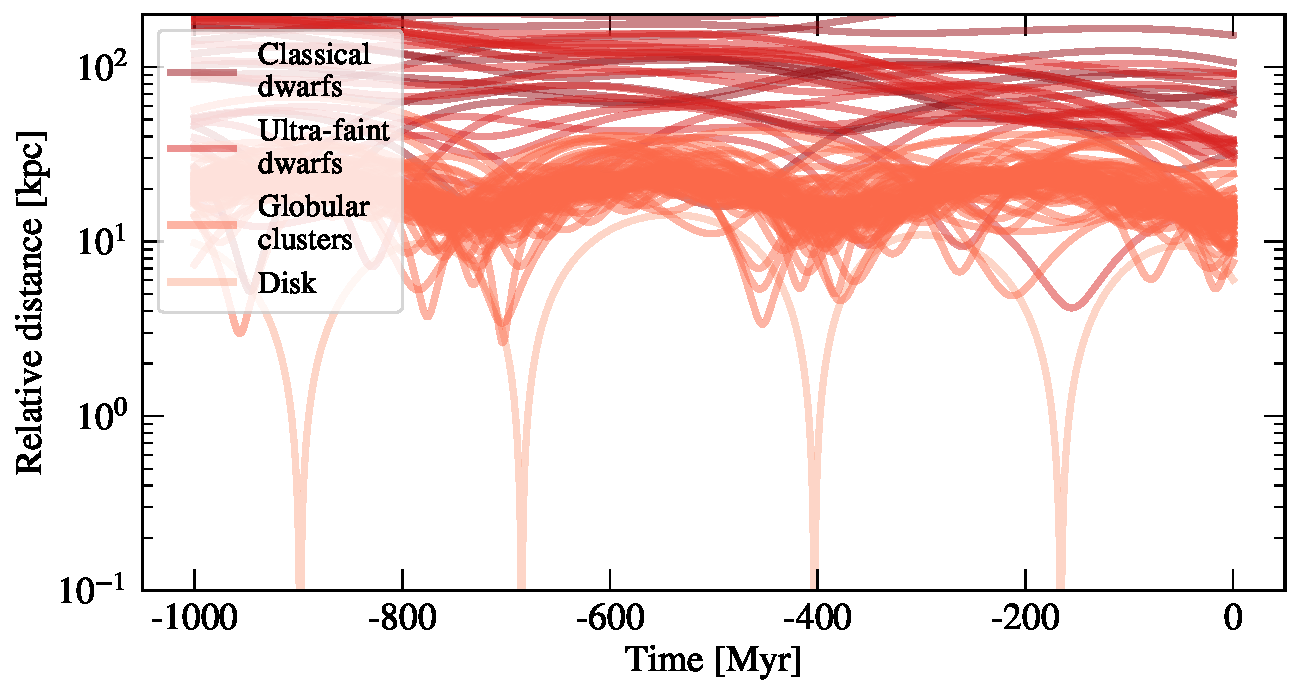
\includegraphics[width=\textwidth]{satellite_distances.pdf}
\end{center}
\caption{Data from \citet{simon2018} and \citet{gdr2_satellites}.}
\label{fig:known_encounters}
\end{figure}

\section{Discussion}

\acknowledgements
It is a pleasure to thank
  Kathryn Johnston (Columbia),
  Adrian Price-Whelan (Princeton),
  and
  Hans-Walter Rix (MPIA)
for valuable discussions and input.
This project was developed in part at the
2018 NYC Gaia DR2 Workshop at the Center for Computational Astrophysics of
the Flatiron Institute in New York City in 2018 April.

This work has made use of data from the European Space Agency (ESA) mission
\Gaia\ (\url{https://www.cosmos.esa.int/gaia}), processed by the \Gaia\ Data
Processing and Analysis Consortium (\acronym{DPAC},
\url{https://www.cosmos.esa.int/web/gaia/dpac/consortium}). Funding for the
\acronym{DPAC}
has been provided by national institutions, in particular the institutions
participating in the \Gaia\ Multilateral Agreement.

\bibliographystyle{aasjournal}
\bibliography{spur}

\end{document}
